\documentclass{exam}
\usepackage[utf8]{inputenc}
\usepackage{lmodern}
\usepackage{microtype}

% \usepackage[parfill]{parskip}
\usepackage[dvipsnames]{xcolor}
\usepackage{amsmath}
\usepackage{amsfonts}
\usepackage{amsthm}
\usepackage{siunitx}
\DeclareSIUnit\year{yr}
\DeclareSIUnit\foot{ft}
\DeclareSIUnit\litre{\liter}

\usepackage{skull}

\usepackage{pgfplots}
\usepgfplotslibrary{polar}
\pgfplotsset{compat=1.11}
\usepgfplotslibrary{statistics}
\usepackage{graphicx}
\usepackage{sidecap}
\sidecaptionvpos{figure}{c}
\usepackage{float}
\usepackage{gensymb}
\usepackage{tkz-euclide}
\usetkzobj{all}
\usepackage{commath}
\usepackage{hyperref}
\usepackage{enumitem}
\usepackage{wasysym}
\usepackage{multicol}
\usepackage{mathtools}
\usepackage{tcolorbox}
\usepackage{tabularx}
\usepackage[version=4]{mhchem}
\usepackage{changepage}
\usepackage{listings}
\lstset{basicstyle=\ttfamily\linespread{0.8}\small}

\renewcommand*{\thefootnote}{\fnsymbol{footnote}}

\newtheorem*{thm}{Theorem}
\newtheorem*{iden}{Identity}
\newtheorem*{lemma}{Lemma}
\newtheorem{obs}{Observation}
\theoremstyle{definition}
\newtheorem*{defn}{Definition}
\newtheorem*{ex}{Example}
\newtheorem{con}{Construction}
\newtheorem*{alg}{Algorithm}

\newtheoremstyle{break}
  {\topsep}{\topsep}%
  {\itshape}{}%
  {\bfseries}{}%
  {\newline}{}%
\theoremstyle{break}
\newtheorem*{bthm}{Theorem}

% russian integral
\usepackage{scalerel}
\DeclareMathOperator*{\rint}{\scalerel*{\rotatebox{17}{$\!\int\!$}}{\int}}

% \DeclareMathOperator*{\rint}{\int}

\pgfplotsset{vasymptote/.style={
    before end axis/.append code={
        \draw[densely dashed] ({rel axis cs:0,0} -| {axis cs:#1,0})
        -- ({rel axis cs:0,1} -| {axis cs:#1,0});
    }
}}

% \pointsinrightmargin
\boxedpoints
\pointname{}

\newcommand{\questioA}{\question[\texttt{\textbf{\color{Cerulean} A}}]}
\newcommand{\questioM}{\question[\texttt{\textbf{\color{PineGreen} M}}]}
\newcommand{\questioE}{\question[\texttt{\textbf{\color{WildStrawberry} E}}]}
\newcommand{\questioS}{\question[\texttt{\textbf{\color{Goldenrod} S}}]}
\newcommand{\questioO}{\question[\texttt{\textbf{\color{BurntOrange} O}}]}

\newcommand{\parA}{\part[\texttt{\textbf{\color{Cerulean} A}}]}
\newcommand{\parM}{\part[\texttt{\textbf{\color{PineGreen} M}}]}
\newcommand{\parE}{\part[\texttt{\textbf{\color{WildStrawberry} E}}]}
\newcommand{\parS}{\part[\texttt{\textbf{\color{Goldenrod} S}}]}
\newcommand{\parO}{\part[\texttt{\textbf{\color{BurntOrange} O}}]}

\newcommand{\subparA}{\subpart[\texttt{\textbf{\color{Cerulean} A}}]}
\newcommand{\subparM}{\subpart[\texttt{\textbf{\color{PineGreen} M}}]}
\newcommand{\subparE}{\subpart[\texttt{\textbf{\color{WildStrawberry} E}}]}
\newcommand{\subparS}{\subpart[\texttt{\textbf{\color{Goldenrod} S}}]}
\newcommand{\subparO}{\subpart[\texttt{\textbf{\color{BurntOrange} O}}]}

\newcommand{\mainHeader}[2]{\section*{NCEA Level 2 Mathematics\\#1. #2}}
\newcommand{\mainHeaderHw}[2]{\section*{NCEA Level 2 Mathematics (Homework)\\#1. #2}}
\newcommand{\seealso}[1]{\begin{center}\emph{See also #1.}\end{center}}
\newcommand{\drills}[1]{\begin{center}\emph{Drill problems: #1.}\end{center}}
\newcommand{\basedon}[1]{\begin{center}\emph{Notes largely based on #1.}\end{center}}


\begin{document}

\mainHeaderDiff{2}{Limits}
How can we define the derivative in such a way that we can calculate with it? Recall that the \textit{average gradient} (or average slope) of
a function $ f $ over the interval $ a \leq x \leq b $ is defined to be $ m = \frac{\Delta y}{\Delta x} = \frac{f(b) - f(a)}{b - a} $. We wish
to find the gradient at a single point; in order to do this, we will slowly move point $ b $ towards point $ a $, letting $ \Delta x $ get closer
and closer to zero. However, we cannot actually let $ \Delta x = 0 $ --- and so we can only ever find an \textit{approximation} to the instantaneous
gradient without a bit of trickery!

Before moving on with the definition of the derivative, let's explore this idea of assigning values to a function by seeing what it looks like
really close to the point we're interested in. We call this operation the \textit{limit}.

Consider the following function:
\begin{center}
  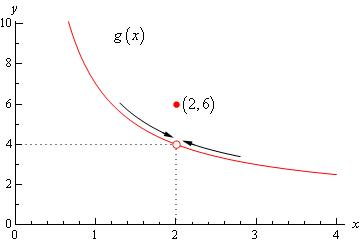
\includegraphics[width=0.5\textwidth]{oslimit2}
\end{center}
Although the \textit{value} of the function at 2 is 6, the \textit{limit} of the function at 2 is $ \lim_{x \to 2} g(x) = 4 $ because when
taking a limit we don't care what the function does at the point --- only what it looks like it should do! Essentially, the
limit of a function at a point is a property of the area around the point \textbf{and not a property of the point itself}.

You can also think of $ \lim_{x \to x_0} f(x) $ as being the unique value that we could pick for $ f(x_0) $ such that the function
around that point has `no gaps'.

\begin{ex}
  Here are a few algebraic examples of limit finding:
  \begin{itemize}
    \item $ \lim_{x \to 0} \frac{x}{x} = 1 $ since as $ x $ gets closer and closer to $ 0 $, $ \frac{x}{x} = 1 $.
    \item $ \lim_{x \to 3} \frac{(x - 2)(x - 3)}{x - 3} = 1 $ since as $ x $ gets closer and closer to 3, the fraction gets arbitrarily close to 1.
    \item $ \lim_{x \to 0} \frac{1}{x} $ does not exist, since if we approach 0 from the left the function becomes arbitrarily negative
          and if we approach 0 from the right the function becomes arbitrarily positive --- we do not approach the same value on both sides.
    \item $ \lim_{x \to \infty} \frac{1}{x} = 0 $ since as $ x $ becomes arbitrarily large, $ \frac{1}{x} $ becomes arbitrarily small.
    \item $ \lim_{x \to 0} \sqrt{x} $ does not exist, since $ \sqrt{x} $ is undefined for $ x < 0 $.
  \end{itemize}
\end{ex}

Now, let's revisit the derivative. We will define the derivative of a function $ f $ at a point $ a $ as
the value of the limit
\begin{displaymath}
  \lim_{h \to 0} \frac{f(a + h) - f(a)}{h},
\end{displaymath}
which is equivalent to the definition above (see exercises).

\begin{ex}
  We will find the derivative of $ f(x) = x^3 $ at the point $ x $ using the definition.
  \begin{align*}
    f'(x) &= \lim_{h \to 0} \frac{f(x + h) - f(x)}{h}\\
          &= \lim_{h \to 0} \frac{(x + h)^3 - x^3}{h}\\
          &= \lim_{h \to 0} \frac{x^3 + 3x^2h + 3xh^2 + h^3 - x^3}{h}\\
          &= \lim_{h \to 0} \frac{3x^2 h + 3xh^2 + h^3}{h}\\
          &= \lim_{h \to 0} 3x^2 + 3xh + h^2\\
          &= 3x^2.
  \end{align*}
\end{ex}

\subsection*{Questions}
\begin{questions}
  \questioA Guess the value of the following limit by evaluating the limuend for each $ x $ in $ \{ \pm 1, \pm 0.5, \pm 0.2, \pm 0.1, \pm 0.05, \pm 0.01 \} $:
            \begin{displaymath}
              \lim_{x \to 0} \frac{\sin x}{x + \tan x}
            \end{displaymath}
  \questioA Consider the function $ f $ graphed below.
    \begin{center}
      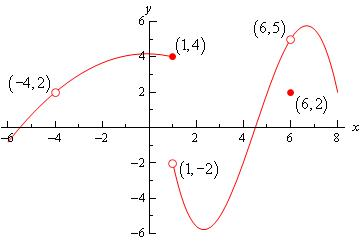
\includegraphics[width=0.4\textwidth]{oslimit}
    \end{center}
    \begin{parts}
      \part For each of the following expressions, either give the value or explain why the expression is undefined.
        \begin{subparts}
          \subpart $ f(-4) $
          \subpart $ \lim_{x \to -4} f(x) $
          \subpart $ f(1) $
          \subpart $ \lim_{x \to 1} f(x) $
        \end{subparts}
      \part Explain why the limit $ \lim_{x \to 6} f(x) $ is not equal to $ f(6) $.
      \part At which points is $ f $:
        \begin{subparts}
          \subpart Discontinuous?
          \subpart Non-differentiable?
        \end{subparts}
    \end{parts}
  \clearpage
  \questioM Evaluate the limit or explain why it does not exist:
    \begin{multicols}{2}
    \begin{parts}
      \part $ \lim_{x \to 2} \frac{x^2 + x - 6}{x - 2} $
      \part $ \lim_{x \to 0} \frac{1}{x^3} $
      \part $ \lim_{x \to 9} \frac{1}{x^3} $
      \part $ \lim_{h \to 0} \frac{(2 + h)^3 - 8}{h} $
      \part $ \lim_{x \to 4} \frac{x^2 + 5x + 4}{x^2 + 3x - 4} $
      \part $ \lim_{x \to \frac{\pi}{2}} \sin x $
      \part $ \lim_{x \to \infty} \sin x $
      \part $ \lim_{x \to \frac{\pi}{2}} \tan x $
      \part $ \lim_{x \to 0} \tan x $
      \part $ \lim_{x \to 0} \csc x $
      \part $ \lim_{x \to a} C $, where $ a $ and $ C $ are constants.
      \part $ \lim_{x \to -\infty} \tan^{-1} x $
      \part $ \lim_{y \to 0} \lim_{x \to 0} \frac{(x + y)(x - y)}{x^2 - y^2} $
      \part $ \lim_{x \to \infty} 1/x $.
      \part $ \lim_{x \to \infty} \frac{2x}{x^2 + 1} $.
      \part $ \lim_{x \to \infty} \frac{x + 2}{x - 3} $.
    \end{parts}
    \end{multicols}
  \questioM Consider the function $ \varphi $ defined by
            \begin{displaymath}
              \varphi(x) = 1/\frac{1}{x - x}.
            \end{displaymath}
            Explain why neither $ \varphi(\alpha) $ nor $ \lim_{x \to \alpha} \varphi(x) $ exists for any real $\alpha $.
  \questioM Find the derivative of $ x^2 + x $ from first principles.
  \questioE Find the derivative of $ \sin x $ from first principles, given that $ \lim_{x \to 0} \frac{\sin x}{x} = 1 $
            and $ \lim_{x \to 0} \frac{1 - \cos x}{x} = 0 $.
  \questioE Show that $ f(x) = \abs{x - 6} $ is not differentiable at $ x = 6 $. Find a formula for $ f' $.
  \questioE Show that $ \lim_{x \to a} \frac{f(x) - f(a)}{x - a} $ and $ \lim_{h \to 0} \frac{f(a + h) - f(a)}{h} $ are
            equivalent definitions for the derivative at the point $ a $ of some function $ f $.
  \questioE If $ \lim_{x \to a} [f(x) + g(x)] = 2 $ and $ \lim_{x \to a} [f(x) - g(x)] = 1 $, find $ \lim_{x \to a} f(x)g(x) $.
  \questioS Consider the following limit (you may assume that it exists):
            \begin{displaymath}
              L = \lim_{n \to \infty} \sum^n_{i = 0} \frac{9}{10^i}
            \end{displaymath}
    \begin{parts}
      \part Write $ L = 0.9 + 0.09 + \cdots $, and make a conjecture about the value of $ L $.
      \part Prove or disprove your conjecture from (a). [\textit{Hint: you may wish to consider the following working.}]
        \begin{displaymath}
          \left(1 - \frac{1}{10}\right)L = 9\left(1 - \frac{1}{10}\right)\left(\frac{1}{10} + \frac{1}{100} + \cdots\right)
        \end{displaymath}
      \part In general, consider the sum $ S_n = \sum_{i = 1}^n ar^i $ for some real constants $ a $ and $ r $. Prove that
        \begin{displaymath}
          \lim_{n \to \infty} S_n = \frac{a(1 - r^n)}{1 - r}.
        \end{displaymath}
        [\textit{Hint: use the same trick as in (b).}] Is there any restriction on $ r $ for this limit to exist?
    \end{parts}
  \clearpage
  \questioS Zeno was a Greek philosopher active in the 5th century BCE. He presented a list of `paradoxes', or apparent contradictions,
            including the following (adapted from Wikipedia):
            \begin{itemize}
              \item Suppose Achilles is in a foot race with a tortoise. Achilles runs much faster than the tortoise, but the latter
                    has a head start. By the time Achilles reaches the location that the tortoise started, the tortoise will have moved
                    a small amount further on; similarly, by the time Achilles reaches the new location of the tortoise, it will have moved
                    an even smaller distance further on; and by this reasoning it follows that Achilles can never overtake the tortoise.
                    \begin{center}
                      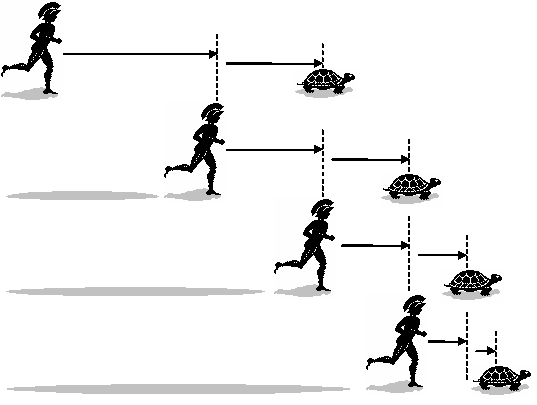
\includegraphics[width=0.4\textwidth]{achilles}
                    \end{center}
              \item Suppose Homer wishes to walk to the end of a path. Before he can get there, he must get halfway there. Before he can
                    get halfway there, he must get a quarter of the way there. Before traveling a quarter, he must travel one-eighth; before
                    an eighth, one-sixteenth; and so on. So Homer cannot walk to the end of the path.
              \item For motion to occur, an object must change the position which it occupies. Consider an example of an arrow in flight. In any
                    one (duration-less) instant of time, the arrow is neither moving to where it is, nor to where it is not. It cannot move to
                    where it is not, because no time elapses for it to move there; it cannot move to where it is, because it is already there.
                    In other words, at every instant of time there is no motion occurring. If everything is motionless at every instant, and
                    time is entirely composed of instants, then motion is impossible.
            \end{itemize}
            Use your knowledge of limits to explain these apparent contradictions.
\end{questions}
\end{document}
